\chapter{Related Work}

\section{Reproducibility of neuroimaging pipelines across operating systems}
Since the claim that ``most published research findings are false” by Ioannidis in 2005 \cite{10.1371/journal.pmed.0020124}, a series of studies have questioned the reproducibility of research results in various disciplines. To mention only a few examples from the neuroinformatics domain, brain activation was found in a dead salmon \cite{BENNETT2009S125}, more than half of the publications in the field of psychology could not be reproduced \cite{aac4716}. The resulting “reproducibility crisis” is challenging the validity of scientific results in several disciplines and we are trying to focus our study on how the operating systems affect the Human connectome project preprocessing pipelines \cite{Gla13}.
 
Neuroimaging pipelines are known to generate different results depending on the computing platform where they are compiled and executed \cite{Gla15}. Such reproducibility issues, also known as computing noise, arise from variations in harware architectures and software versions. The state-of-the-art solution to deal with these issues is to restrict studies to a single computing platform (harware and software), which has several drawbacks and, therefore, not feasible. So the best approach is to become aware of these differences.

Study conducted on FSL, Freesurfer and CIVET and different versions of GNU/Linux \cite{Gla15} shows that the differences are occuring due to the evolution of math libraries used in the operating system on which the processing takes place. A similiar study \cite{10.1371/journal.pone.0038234} concludes that the operating system updates and the software updates itself can cause differences in the results of neuroimaging pipelines. We are tying to identify the reasons that causes these differences.\\

Explain differences.\\

\section{Potential causes of differences}
The issues regarding reproducbility could arise due to a variety of reasons other than the evolution of math libraries. The way in which the build takes place(static vs. dynamic),the nature of the language(compiler vs. interpreter), the version of the compiler used, the options used while compiling the code etc.\\ 

\section{Containers}
The serious challenge associated with making an experiment reproducible is the rapidly changing nature of computer environments. Containers help in encapsulating of the complete software environment. Our study focus on quantifying the effect of operating system on the neuroimaging pipelines. For the ease of conducting experiments across different operating systems/versions, we containerized the different operating systems\footnote{\url{https://hub.docker.com/u/bigdatalabteam}} along with the neuroimaging pipelines that are required for conducting the experiments	. Some of the notable features of containers \cite{docker-run} \cite{DBLP:journals/corr/HaleLRW16} \cite{Julian:2016:CRI:2949550.2949562} \cite{10.1109/ISPASS.2015.7095802} which would help running the experiments with ease are listed below:

\begin{itemize}
  \item Helps in encapsulating the entire software environment
  \item Avoids the software version conflicts with the host os by packaging the right software versions and dependencies in the container environment
  \item Simplified collaboration and sharing ability
  \item Improved reproducibility and portability of applications
  \item Host OS agnostic
  \item Rapid deployment and execution at scale  
\end{itemize}

Container is similiar to a virtual machine, but it uses the same host operating system along with a container manager where as traditional virtual machines needs significant amount of resources to run a virtual machine even if it is not being used. It might take up several gigabytes of memory from the host operating system for running virtual machine \cite{DBLP:journals/corr/HaleLRW16}. Container technologies has been around for a while and there are numerous implementations of it. In the year 2000, FreeBSD (4.0) featured the Jails system which focused on providing an isolated filesystem. Later came OpenSolaris, providing not only isolation services but also mechanisms related to snapshots and cloning. In 2005, OpenVZ was announced as a containerization technology supporting Linux systems. Linux containers (LXC), took advantage of the namespace concept. LXC extended the isolation property to users, processes and networking. In 2006, Google started a project which implemented a functionality to limit the resource usage. This project was later merged into the Linux kernel and it was named as "cgroups" feature. \\
 
``Control cgroups, usually referred to as cgroups, are a Linux kernel feature which allow processes to be organized into hierarchical groups whose usage of various types of resources can then be limited and monitored" \cite{cgroups}. Docker, was started as an open source project in 2013, which basically added an additional layer on top of LXC, exposing additional features such as mounted storage, network port redirection, and container catalog management. Singularity, was started in 2015, with main focus on experimental reproducbility and isolation \cite{Xavier:2013:PEC:2497369.2497577}.\\ 

Containers have a closer access to operating systems than their counterpart virtualization tools such as native virtualization, paravirtualization, and hypervisors. In native virtualization, also known as full virtualization, the guest OS is fully abstracted (completely decoupled) from the underlying hardware by the virtualization layer. Paravirtualization involves modifying the OS kernel to replace nonvirtualizable instructions with hypercalls (a hypercall is a way for the virtualized operating systems to make the hypervisor handle privileged operations) that communicate directly with the virtualization layer hypervisor \cite{citeulike:11530382}. Non-virtualizable instructions are instructions on X86\footnote{\url{https://en.wikipedia.org/wiki/X86}} architecture that are sensitive but are not privileged \cite{non-virtualizable-commands}.\\ 

``Hypervisor also known as Virtual Machine Monitor (VMM), is the basic software for providing virtualization. Virtualization creates the environment for various operating system to run on a single node or host computer or machine. The main purpose of the hypervisor (VMM) is to monitor the Virtual Machine (VM) that runs above the VMM. This enables more than one guest machine to utilize the hardware resources of a single host machine" \cite{hypervisor}. Containers subtract the hypervisor layer and accesses the host operating system features directly making it lightweight.\\

\begin{center}
\begin{minipage}{0.48\linewidth}
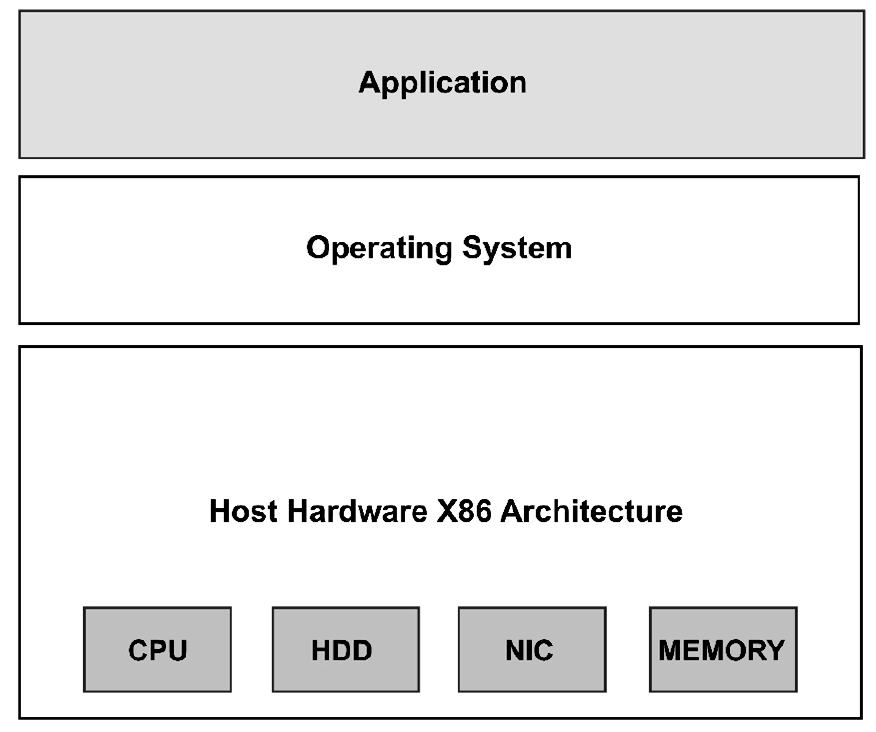
\includegraphics[height=8cm,width=\linewidth]{no_virtualization.png}
\captionof{figure}{Machine with no virtualization}
\label{fig:novirtualization}
\caption*{Extracted from \cite{10.4236/ijcns.2015.87026} Figure 2}
\end{minipage}%
\hfill
\begin{minipage}{0.48\linewidth}
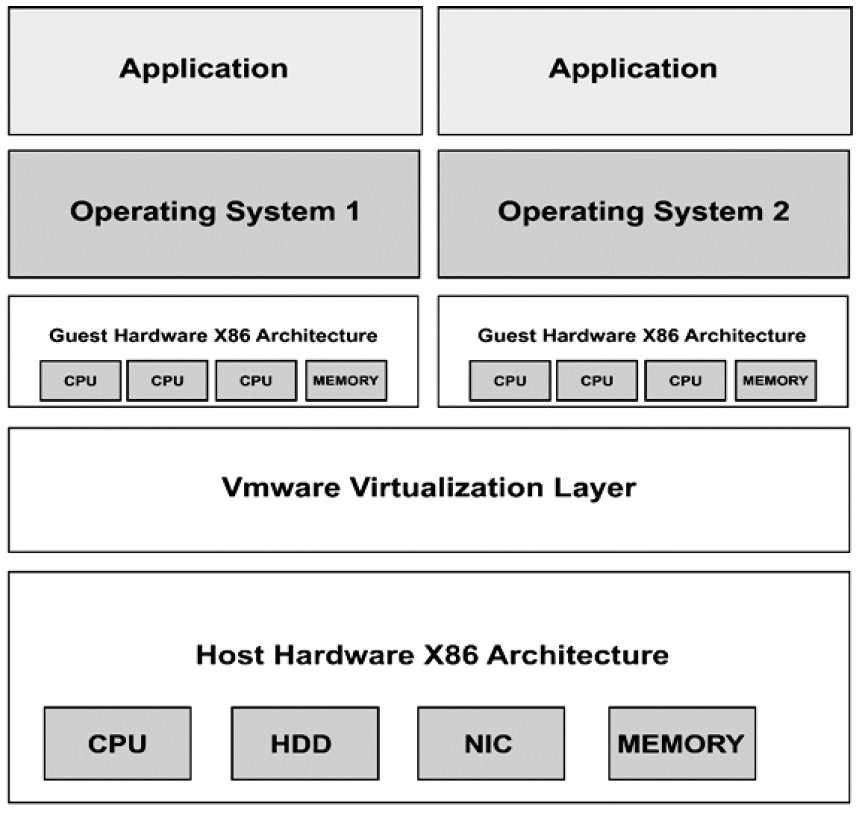
\includegraphics[height=8cm,width=\linewidth]{with_virtualization.png}
\captionof{figure}{Machine after virtualization}
\label{fig:aftervirtualization}
\caption*{Extracted from \cite{10.4236/ijcns.2015.87026} Figure 3}
\end{minipage}
\end{center}

These containers allow a user to run application and its dependancies in resource-isolated processes. Containers have a closer access to operating system services than their counterpart virtualization tools which makes their performance closer to the performance exhibited on top of native environments\cite{Xavier:2013:PEC:2497369.2497577}.\\

Even if we get access the software and tools used in an experiment, it is extremely hard to reproduce the workflow due to many undocumented assumptions, dependencies, and configurations \cite{7883438}. Containers can help in recreating the software environment used for the experiment in its entirety. This can help the researchers significantly since they don't have to go through the entire process of installation process. ``Docker" and ``Singularity" are two container based technologies widely used for containerizing the applications.\\

What are its limitations
Include the problems listed in link https://goo.gl/zodrok

\subsection{Docker}
Docker provides access to virtualization facilities provided by the Linux kernel, along with some abstracted virtualized interfaces such as libvirt\footnote{\url{https://libvirt.org/}}, LXC and systemd-nspawn\footnote{\url{https://www.freedesktop.org/software/systemd/man/systemdnspawn.html}}. The control over the host's resources is provided thorugh Control Groups(cgroups) and thus it limits the amount of resources used by a container such as memory, diskspace and I/O. Docker features a layered filesystem called AuFS(Advanced Multi Layered Unification Filesystem) which allows to overlay one or more existing filesystems. This AuFS feature provides capabilites such as image versioning management and exposing base images to more specialized virtualized systems. One of the main reason for the wide adoption of docker containers is that it can leverage the infrastructure consolidation and it exhibits a low resource footprint. Docker also boosted the adoption of service oriented architectures (e.g. microservices) because that makes the deployment of self-contained modules easy. They are also able to independantly interact with third parties using exising network protocols (e.g. web services) \cite{Xavier:2013:PEC:2497369.2497577}. \\

The Docker software runs as a daemon on host machine. This daemon can launch containers, control their isolation level, monitor them to trigger actions, and spawn shells into running containers for administration purposes. Daemon can change iptable rules on the host and create network interfaces. The management of the images on the host machine, pushing and pulling of images from Dockerhub\footnote{\url{https://www.hub.docker.com/}}, building images from Dockerfile are all taken care by the daemon. The daemon itself runs as a root user on the host machine and it is remotely controlled through a Unix socket. Docker useas a client-server architecture.The Docker client talks to the Docker daemon and the daemon does all the heavy lifting like pushing, pulling and building images.The Docker client and daemon communicate using a REST API, over UNIX sockets or a network interface. The client and daemon need not necessarily be on the same machine\cite{docker-documentation}.

\begin{center}
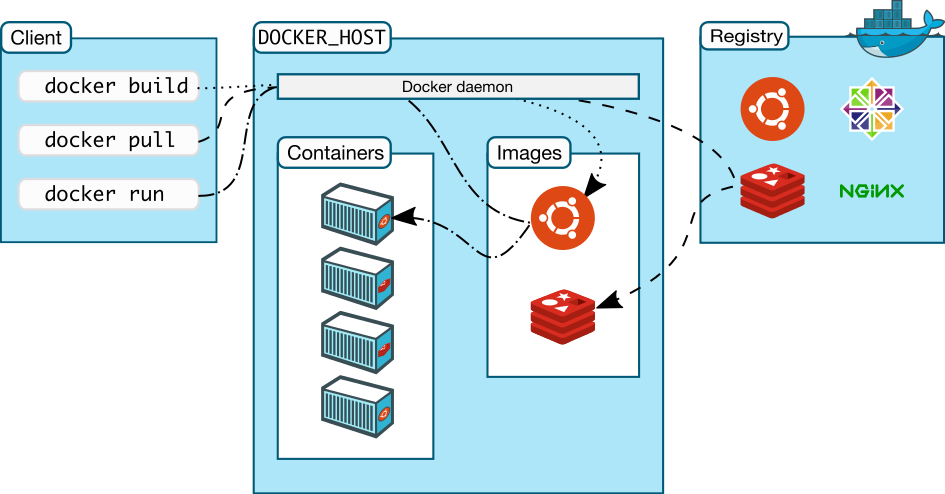
\includegraphics[width=\linewidth]{docker_architecture.png}
\captionof{figure}{Docker Architecture}
\label{fig:docker_architecture}
\caption*{Extracted from \cite{docker-documentation}}
\end{center}

The Dockerhub is an online repository that helps developers to manage the images. Anyone who sign up on the docker hub has access to images where they can push or pull images. There is also feature for making the image creation automated with the help of git technology. Any user can create repository under his account and the repositories are namespaced using the format, "\textless developer\textgreater/\textless repository\textgreater"\cite{7742298}.\\

The wide adoption of docker containers can be attributed to both the speed and simplicity of Docker containers. The development of standardized Dockerfile format for describing and managing software containers is very straightforward. Docker helps developers to easily create standard containers for their software applications or services. For a system administrator, Docker helps in the automation of depolyment and management of business level services with the help of containers. Docker can be used as a part of virtualization layer for deploying and managing the execution environments. Another advantage is that docker containers provide reliable and predicatable execution environments and thus helps in reducing the issues related to deployment \cite{DBLP:journals/corr/MorrisVHM17}.

\subsection{Singularity}
``Singularity is an open source initiative that harnesses the expertise of system and software engineers and researchers alike, and integrates seamlessly into common workflows for both of these groups. One of the major reason for this this open source initiative started by the Lawrence Berkeley National Laboratory (LBNL) was that, if Docker is used on HPC environments, that would mean an unreasonable level of security risk. So Docker could not be used by a large group of people that needed it greatly. Thus Singularity open source initiative came up with a product that could be used across academia and industry which is agnostic to the environment. It was developed in collaboration by HPC administrators, developers and research scientists alike. The main issue with docker running on the HPC clusters was that the daemon has to run as a root user which could lead to unnecessary risks like coercing the daemon process into granting the users escalated privileges" \cite{10.1371/journal.pone.0177459}.\\

\begin{center}
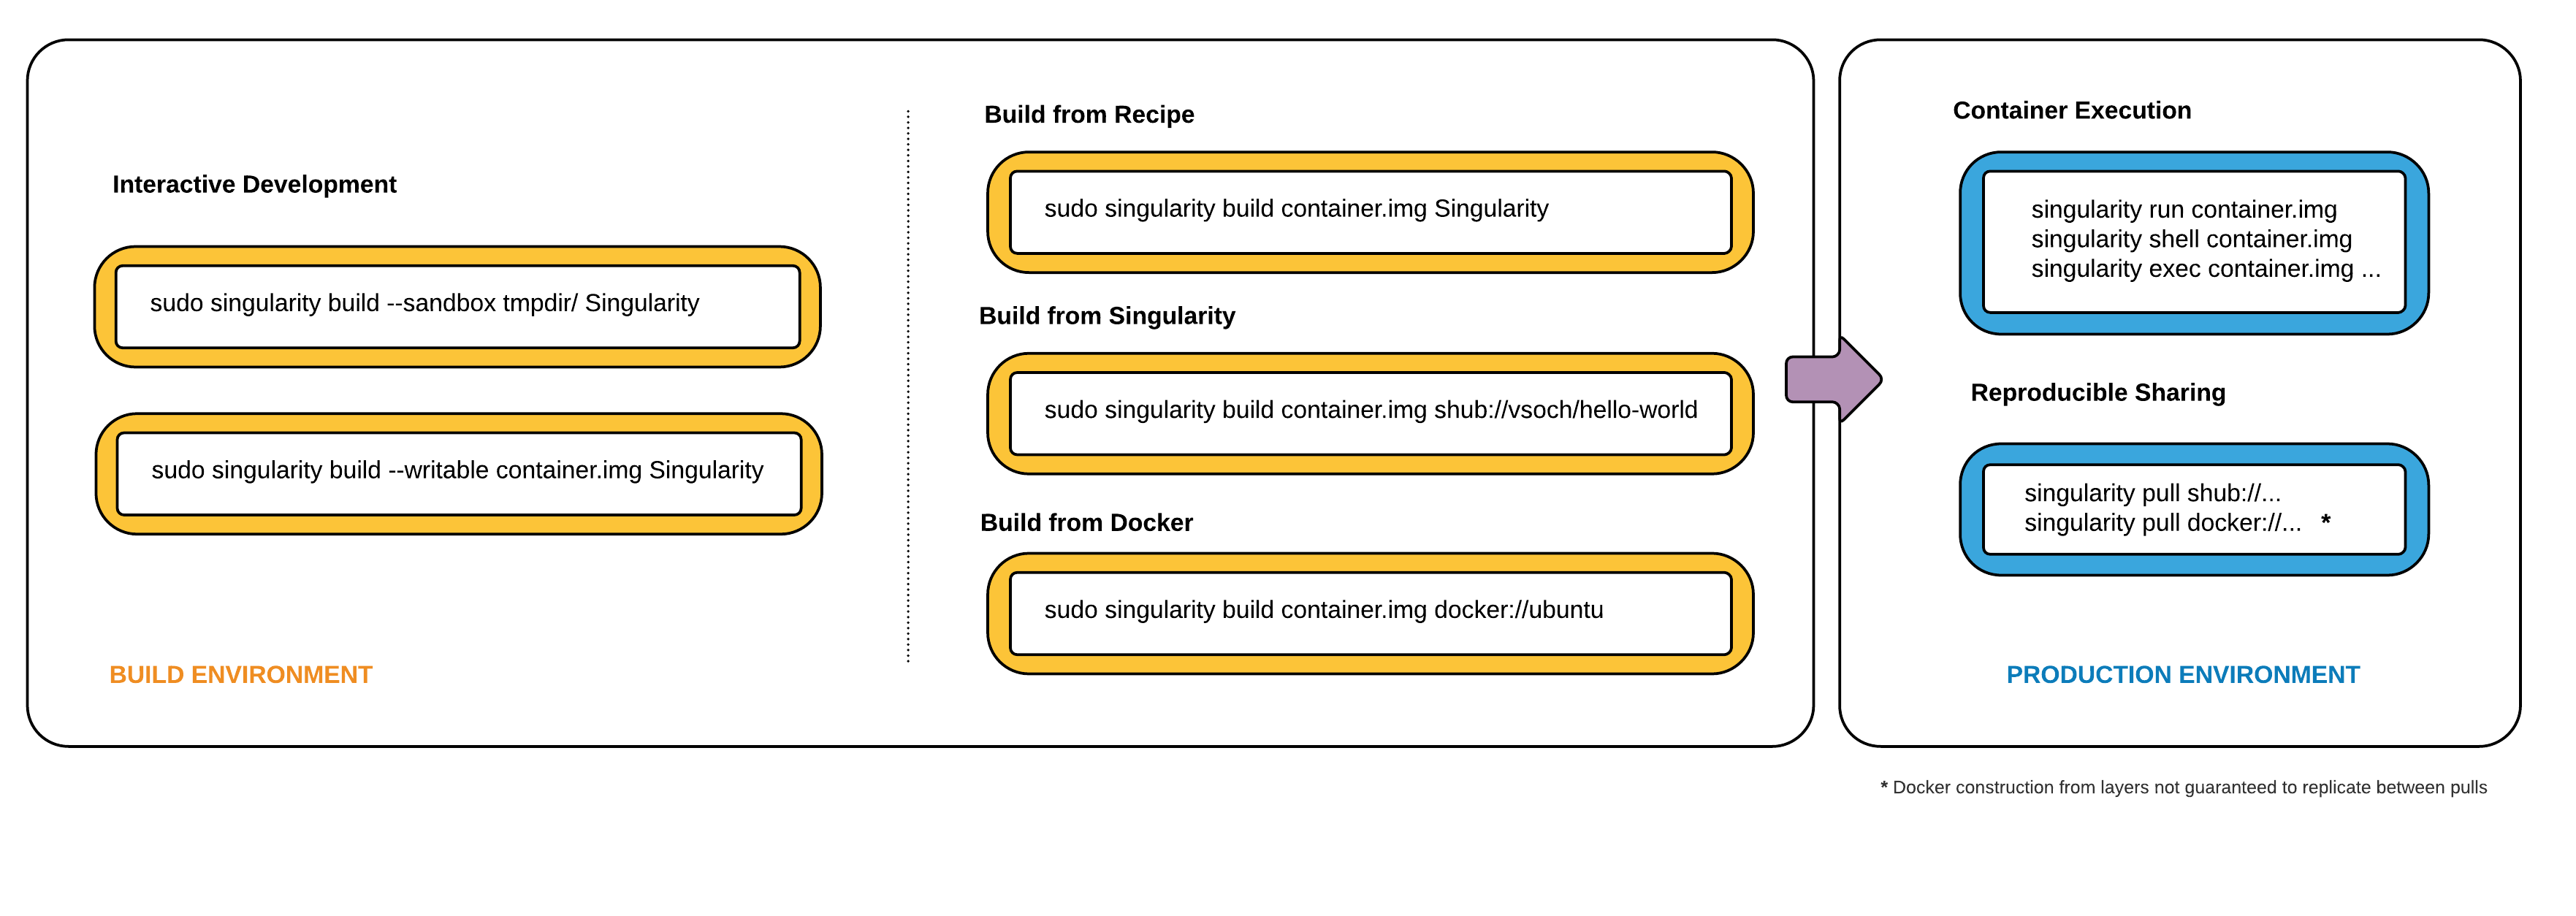
\includegraphics[width=\linewidth]{singularity.png}
\captionof{figure}{Singularity usage workflow.}
\label{fig:singularity_workflow}
\caption*{Extracted from \cite{10.1371/journal.pone.0177459}}
\end{center}

The main goals of Singularity are, 1)Mobility of compute 2)Reproducibility 3)User Freedom 4)Support on existing traditional HPC resources. The mobility of compute is the ability to create and maintian a workflow locally and being able to run the same worklfow across different hosts, operating systems or computing platforms without any problems or tweaks. Singularity achieves this by utilizing a distributable image format that encapsulates the entire container and stak into a single image file. The feature that supports reproducibility is the use of hashing. Any singularity image can make use of the hash feature to create hash and store it as metadata with built images. Users can verify these hashes to check if the image is modified or not. User freedom is granted by the ability to define their own working environment and copy the singularity image containing the entire details of that environment along with the code to a shared resource and reproduce the workflow inside that image. Singularity supports the existing and traditional HPC resources easily as installing a single package onto host operating system. Singularity is compatible with RHEL and Linux distributions dating back to Linux2.2. It natively supports the resource managers(e.g SLURM\footnote{\url{https://slurm.schedmd.com/}}(a free and open-source job scheduler for Linux and Unix-like kernels),Torque\footnote{\url{http://www.adaptivecomputing.com/products/open-source/torque/}}(Open-source Resource and QUEue Manager is a distributed resource manager providing control over batch jobs and distributed compute nodes), SGE\footnote{\url{https://en.wikipedia.org/wiki/Oracle_Grid_Engine}}(A grid computing computer cluster software system), etc.) and supports technologies such as InfiniBand\footnote{\url{https://en.wikipedia.org/wiki/InfiniBand}}(A computer-networking communications standard used in high-performance computing that features very high throughput and very low latency) and Lustre\footnote{\url{https://en.wikipedia.org/wiki/Lustre_(file_system)}}(Open source, parallel file system that supports many requirements of leadership class HPC simulation environments).\\

Singularity container image encapsulates the operating system environent and all application dependencies necessary to run a defined workflow. Singularity container supports different kinds of uniform resource identifiers and also other container formats like Docker. http://,https://,docker://(for pulling images from docker hub),shub://(for pulling images from singularity hub), all these mechanisms are supported by singularity for obtaining the images. One another notable feature of Singularity is that it does not provide a pathway for privilege escalation. At runtime, a user inside the Singularity container has the same role and privileges as the user outside the container.
 
\subsection{Boutiques}
To enable sharing of ideas and software, it is a common practise to port the applications to common platforms so that the community as a whole is able to make use of the ready-to-use applications. However, porting applications to a high performance computing infrastructure or a web platform is not so easy. Application porting needs considerable effort of manual effort to `` 1) install the application on the target infrastructure, 2) describing the application in a format compatible with the execution platform, and 3) generating proper user interfacesi" \cite{boutiques}. These installations and deployments are platform specific and thus the same tasks has to be repeated from one platform to another. Boutiques, an open source tool, can be used to save time and cost spent on these repeated actions to deploy applications on various platforms. \\

``Docker and Singularity, greatly facilitate the sharing of software and improve the reproducibility of analysis by defining immutable, reusable execution environments" \cite{boutiques}. The software or applications inside these containers should be invoked through proper command line to run an application. Boutiques makes use of a flexible template that could properly describe the inputs and outputs an application produces. ``The formal descriptions, also known as \textit{manifests}, are used for validation of input values to prevent errors. These manifests are intended to be produced by scientific application developers, for publishing them in common repositories and to be consumed by execution platforms". The preferred way of describing these command line template, input and argument is through a JSON document. The manifest contains the details to a container where the intended application is installed. The proper command line argument is built at runtime with the help of maifest and the template gets replaced by the actual values given by the user. For validating the inputs an invocation schema is used. \\

Here is an example of a typical command-line template:

\begin{verbatim}
          exampleTool [INPUT-FILE] [OUTPUT_FILE]
\end{verbatim}

The command line above invokes a tool named exampleTool that needs an two arguments, an input file and an output-folder.
``\textit{Inputs} must have a name, a unique identifier and a type. They may be optional, have a description, a value key, a flag separator, and a default value. Inputs may also be ordered lists: in this case, value keys are substituted by the space-separated list of input values. \textit{Output} files must have a unique identifier, a name and a path template that specifies the file or directory name" \cite{boutiques}.

At runtime, with the help of the JSON descriptor, Boutiques substitutes all the mandatory parameters and the optional parameters with the original values selected by the user. The core tools of Boutiques are validator and local executor. Boutiques validator checks if the JSON manifests confirm to the rules of Boutiques schema. And local executor can be used to test and debug the applications locally.

\begin{center}
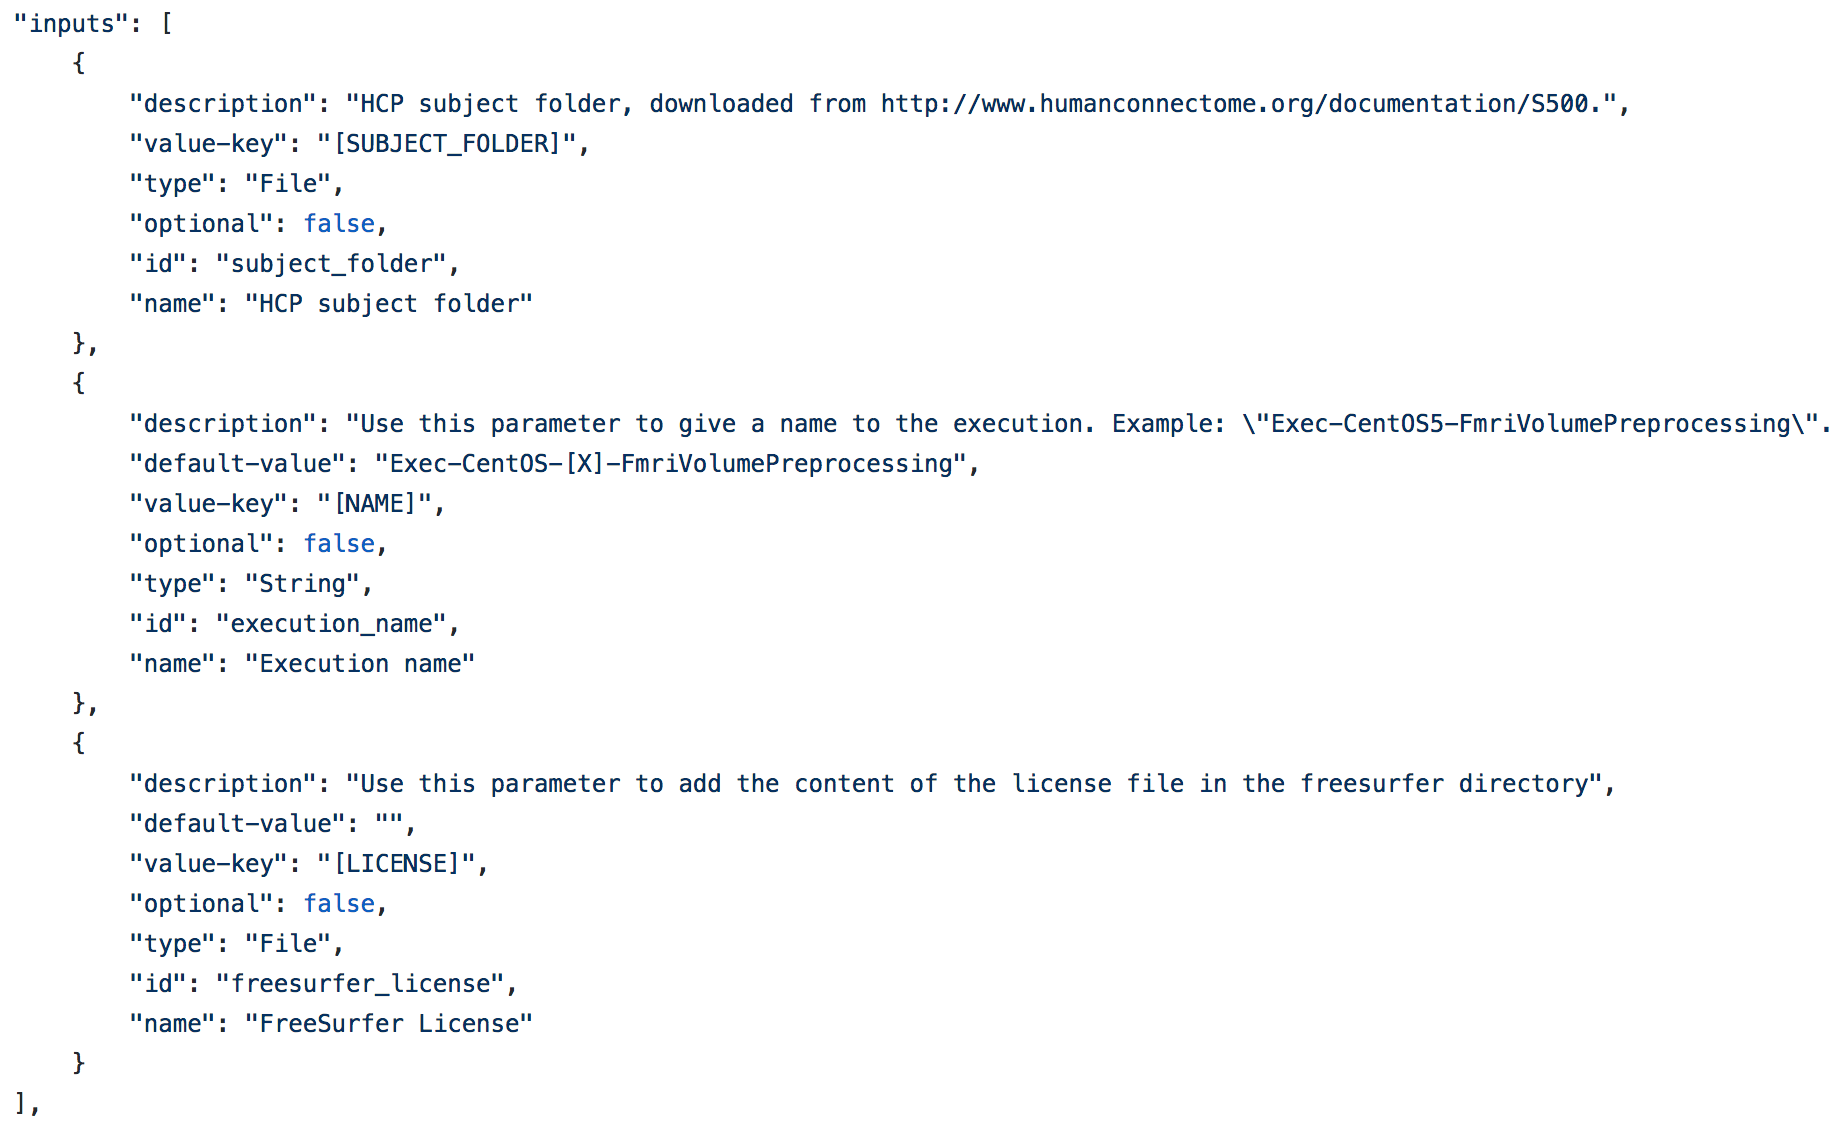
\includegraphics[width=\linewidth]{input.png}
\captionof{figure}{Boutiques input descriptor.}
\label{fig:input}
\end{center}

\begin{center}
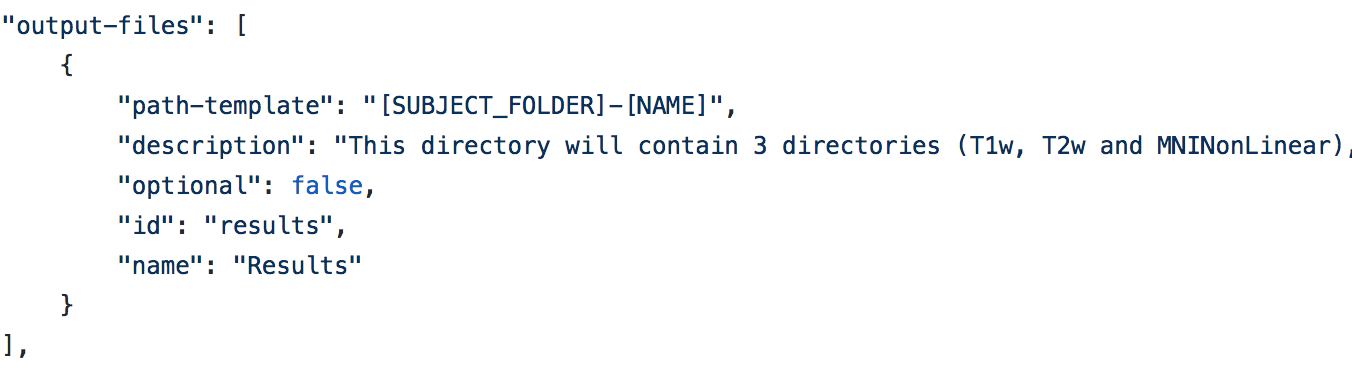
\includegraphics[width=\linewidth]{output.png}
\captionof{figure}{Boutiques output descriptor.}
\label{fig:output}
\end{center}



\section{Web platforms to run containers}
\subsection{Why do we need these platforms?}
\subsection{Examples of web computing platforms}
\subsubsection{CBRAIN}
\subsubsection{Amazon}

\section{Interposition Techniques}
\subsection{System call interception}
\subsection{Library call interception}
\subsection{Reprozip tool}
\hyperref[System Call Interception]{http://landley.net/kdocs/mirror/ols2007v1.pdf}

\section{NeuroImaging Pipelines}
The Human Connectome Project(HCP) faces the challenging task of bringing multiple magnetic resonance imaging(MRI) modalities, structural, functional, and diffusion,together into a common automated preprocessing framework across a large cohort of subjects. This framework is open and freely accessible \cite{Gla13}. The dataset from the HCP, are qualitatively different from standard neuroimaging data, having higher spatial and temporal resolutions and differing distortions. So these preprocessing pipelines creates preprocessing results that are available in standard volume and combined surface and volume spaces which makes it easier for researchers to compare the images across the neuroimaging spectrum. Since the images from the HCP dataset are cutting edge in terms of quality, it is anticipated to be widely used.

HCP minimal preprocessing pipelines are designed to minimize the amount of information actually removed from the data. These pipelines are dependant on the underlying operating system libraries for many of its functions. Hence, when there are updates in operating system versions, there could be changes in the ways which the rounding off and truncation of floating-point numbers are handled. We are trying to quantify the differences occuring due to the operating system updates on HCP preprocessing pipelines.

\begin{itemize}
 \item FSL
 \item FreeSurfer
 \item HCP Pipelines
\end{itemize}


